% This must be in the first 5 lines to tell arXiv to use pdfLaTeX, which is strongly recommended.
\pdfoutput=1
% In particular, the hyperref package requires pdfLaTeX in order to break URLs across lines.

\documentclass[11pt]{article}

% Remove the "review" option to generate the final version.
\usepackage[review]{acl}

% Standard package includes
\usepackage{times}
\usepackage{latexsym}

% For proper rendering and hyphenation of words containing Latin characters (including in bib files)
\usepackage[T1]{fontenc}
% For Vietnamese characters
% \usepackage[T5]{fontenc}
% See https://www.latex-project.org/help/documentation/encguide.pdf for other character sets

% This assumes your files are encoded as UTF8
\usepackage[utf8]{inputenc}

% This is not strictly necessary, and may be commented out,
% but it will improve the layout of the manuscript,
% and will typically save some space.
\usepackage{microtype}

% If the title and author information does not fit in the area allocated, uncomment the following
%
%\setlength\titlebox{<dim>}
%
% and set <dim> to something 5cm or larger.

%algo packages
\usepackage{algorithm}
\usepackage{algorithmic}

%color packages
\usepackage{xcolor}
\colorlet{shadecolor}{orange!15}
\usepackage{color,soul}
\usepackage{soulutf8}
\definecolor{bordeau}{rgb}{0.3515625,0,0.234375}

% position of figure
\usepackage[absolute,overlay]{textpos}

%graphic packages
\usepackage{graphicx}
\graphicspath{ {figures/} }
\usepackage{wrapfig}
\usepackage{float} 
\usepackage{tikz}
\usepackage{pgfplots}
\usepackage{pgfplotstable}

% table packages
\usepackage{array}
\usepackage{multirow,booktabs}
\usepackage{multicol}
\usepackage{tabularx}

% font package
\usepackage[utf8]{inputenc}	% Para caracteres en español
\usepackage{textcomp}
%\usepackage{times}
%\usepackage{lmodern}
\usepackage{mathptmx}

% equation packages
\usepackage{amsmath,amsthm,amsfonts,amssymb,amscd}
\usepackage{mathrsfs}

\usepackage{enumitem}
\setlist{nosep}
\usepackage{latexsym}
\usepackage{graphicx}
\usepackage{xcolor}
\usepackage{longtable}
\usepackage{tikz}
\usetikzlibrary{calc}
\usepackage[draft]{todo}
\usepackage[normalem]{ulem}
\usepackage{xspace}
\usepackage{amsmath,amsfonts,amssymb}

\newcommand{\fyTodo}[1]{\Todo[FY:]{\textcolor{orange}{#1}}}
\newcommand{\fyTodostar}[1]{\Todo*[FY:]{\textcolor{orange}{#1}}}
\newcommand{\fyDone}[1]{\done[FY]\Todo[FY:]{\textcolor{orange}{#1}}}
\newcommand{\fyFuture}[1]{\done[FY]\Todo[FY:]{\textcolor{red}{#1}}}
\newcommand{\fyDonestar}[1]{\done[FY]\Todo[FY:]{\textcolor{orange}{#1}}}
\newcommand{\jcTodo}[1]{\Todo[JC:]{\textcolor{red}{#1}}}
\newcommand{\jcDone}[1]{\done[JC]\Todo[JC:]{\textcolor{red}{#1}}}
\newcommand{\revision}[1]{\textcolor{black}{#1}}
\newcommand{\revisiondone}[1]{\textcolor{black}{#1}}
\newcommand{\revisiondel}[1]{}
\newcommand{\src}{\ensuremath{\mathbf{f}}} % source sentence
\newcommand{\trg}{\ensuremath{\mathbf{e}}} % target sentence
\newcommand{\domain}[1]{\texttt{\textsc{#1}}}
\newcommand{\system}[1]{\texttt{{#1}}}
\newcommand{\SB}[1]{\textbf{#1}}
\newcommand{\SW}[1]{\underline{#1}}


\title{Multi-domain, multilingual translation with latent multi-task group dropout}

% Author information can be set in various styles:
% For several authors from the same institution:
% \author{Author 1 \and ... \and Author n \\
%         Address line \\ ... \\ Address line}
% if the names do not fit well on one line use
%         Author 1 \\ {\bf Author 2} \\ ... \\ {\bf Author n} \\
% For authors from different institutions:
% \author{Author 1 \\ Address line \\  ... \\ Address line
%         \And  ... \And
%         Author n \\ Address line \\ ... \\ Address line}
% To start a seperate ``row'' of authors use \AND, as in
% \author{Author 1 \\ Address line \\  ... \\ Address line
%         \AND
%         Author 2 \\ Address line \\ ... \\ Address line \And
%         Author 3 \\ Address line \\ ... \\ Address line}

\author{First Author \\
  Affiliation / Address line 1 \\
  Affiliation / Address line 2 \\
  Affiliation / Address line 3 \\
  \texttt{email@domain} \\\And
  Second Author \\
  Affiliation / Address line 1 \\
  Affiliation / Address line 2 \\
  Affiliation / Address line 3 \\
  \texttt{email@domain} \\}

\begin{document}
\setlength{\parskip}{0pt}
\setlength{\abovedisplayskip}{0pt}
\setlength{\belowdisplayskip}{0pt}
\setlength{\abovedisplayshortskip}{0pt}
\setlength{\belowdisplayshortskip}{0pt}
\maketitle
\begin{abstract}
Multi-domain and multilingual translation can be cast under multi-task learning in which each domain or language pair is considered a task. Sharing most of the parameters of the model causes a catastrophic interference between unrelated tasks. Most of the proposed multi-task architectures propose sharing the parameters of an underlying generic model and using different output layers to predict different tasks. However, these methods do not explicitly exploit the proximity between tasks. In this work, we aim to express the task proximity in the multi-task network. Instead of using a predefined multi-task network, we jointly learn routing task-dependent sub-networks and the parameters of the whole network. More precisely, we propose clustering the nodes of each layer into equal-sized groups. For each layer and each domain, a number of groups will be dropped. By consequence, we assign different sparse sub-networks to different tasks. Our method learns the task-dependent dropping selections and the parameters of the underlying network. Our approach allows the proximity between tasks to express in their dropping selections. Through an extensive set of experiments, we demonstrate the advantages of our method over strong baselines in multi-domain and multilingual translation. Furthermore, through an ablation study, we illustrate a significant correlation between the similarity between learned task-dependent dropping selections and the proximity between tasks.
\end{abstract}

\section{Introduction}
Multi-domain translation and multilingual translation develop one model for translations in multi-domain and multiple language pairs, respectively. These paradigms are motivated by the compactness of the translation model \cite{dabre20survey,Chu18multilingual} and the hypothetical positive knowledge transfer between similar domains \citep{Pham21revisiting} or between languages in the same family \citep{Tan19multilingual}. However, sharing parameters of the model can cause the catastrophic interference between unrelated tasks \citep{conneau20unsupervised,wang20negative}.

In multi-domain setting, \citet{Pham21revisiting} pointed out a challenge in how multi-domain systems fully exploit the similarity between domains. The authors demonstrated the weakness of these systems in handling the proximity between domains through a simple setting using a pseudo domain separation. Domain Adapters, which are strong baselines for multi-domain translation \cite{Pham20Study}, failed this test. Such predefined allocations of parameters to domains do not take into account the proximity of domains in their choice.

The method we developed here mitigates the catastrophic interference in training a neural machine translation (NMT) model for multiple domains or multiple language pairs. Our main contribution are summarized below:
\begin{itemize}
\setlength{\itemsep}{1pt}
  \setlength{\parskip}{0pt}
  \setlength{\parsep}{0pt}
	\item We provide a rigorous mathematical modeling the problem of jointly learning routing task-dependent sub-network and the parameters of the underlying model using variational probabilistic modeling.
	\item Our method propose end to end training with very little extra computational cost.
	\item With an extensive experimental setting, we demonstrate a significant gain of our method against strong baselines.
	\item We illustrate a significant correlation between the similarity between learned sub-networks and the proximity of their corresponding tasks.
\end{itemize}

\section{Multi-task group dropout}
We define a group dropout for a domain $d$ as follows
\begin{align*}
\tilde{h}^l &= h^l \odot r_l^d ,\\
r_l^d &\in \{ 0,1 \}^{d_k}, \\
h^{l+1} &= \text{LAYER}^{l+1}(h^l) ,\\
l & \in [0,\cdots,L] ,\\
\end{align*}
where $L$ is number of Transformer layers of our NMT model, the binary vector $r_l^d$ is a dropping mask. We illustrate the group dropout in Figure \ref{fig:group_dropout}
\begin{figure}
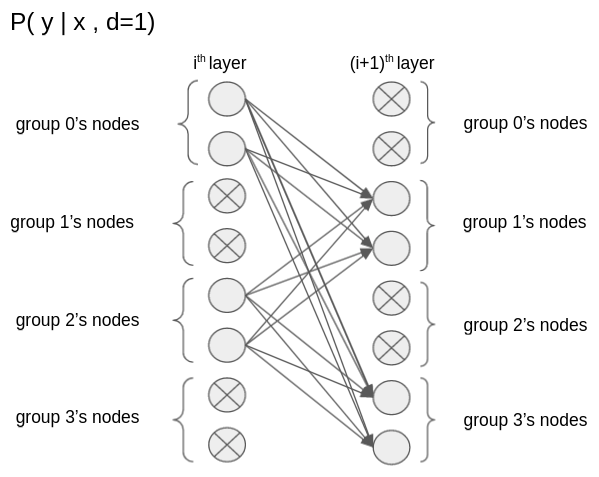
\includegraphics[width=0.4\textwidth]{group_dropout}
\caption{Latent group dropout. The set of nodes in one layer is divided into equal-sized groups. For a domain, we drop a fixed number of groups. Our method learns which groups will be dropped for a domain.}
\label{fig:group_dropout}
\end{figure}
 The dropping mask $r_l^d$ of $l^{th}$ layer and domain $d$ is defined as follows
\begin{align*}
r_l^d(i) &= \begin{cases}
      1, & \text{if}\ p \times \frac{d_k}{n_p} \leqslant i < (p+1) \times \frac{d_k}{n_p} \\
      & \text{AND} \  m_l^d(p) \text{\small ==} 1 \\
      0, & \text{otherwise},
    \end{cases} \\
p & \in  \{0,\dots,n_p\text{-}1 \}, \\
d & \in  \{0,\dots,n_d\text{-}1 \}, \\
i & \in  \{0,\dots,d_k\text{-}1 \}, \\
m_l^d & \in  \{0,1\}^{n_p} \ \forall d,l \, \\
\mid m_l^d \mid_{L_1} & =  k , \\
\Delta^{n_p}_k & =  \{ m \in \{0,1\}^{n_p} | \mid m \mid_{L_1} = k \},
\end{align*}
where $n_p$ is the number of dropout groups; $n_d$ is the number of domains; $d_k$ is the size of Transformer layers; $k$ is the number of retained groups at each layer; $m_l^d$ is a binary vector indicating which group of the nodes of the $l^{th}$ layer is dropped in the sub-network modeling domain $d$. The group $p$ is retained for domain $d$ if $m_l^d(p)\text{\small ==}1$ and is dropped if $m_l^d(p)\text{\small ==}0$. We also denote $\Delta^{n_p}_k$ the set of all admissible dropping masks. 

We incorporate the latent variables $m_{l\in[0,\cdots,L]}^d$ into the log-likelihood of our model as below. For the sake of brevity, we denote $m_l^d$ the set of latent variables $m_{l\in[0,\cdots,L]}^d$
\begin{align}
\hspace{-3.em}
\text{log} P(y|x,\theta,d) & \text{=} \text{log} P(y, m_l^d |x,\theta,d) \text{-} \text{log} P(m_l^d|y, x,\theta,d) \nonumber \\
& \text{=} \displaystyle{\mathop{\mathbb{E}}_{P(m_l^d | \Phi_l^d)}} \big[ \text{log} P(y, m_l^d | x,\theta,d) \text{-} \text{log} P(m_l^d | \Phi_l^d) \big] \nonumber \\
& \text{+} KL(P(m_l^d | \Phi_l^d) \parallel P(m_l^d|y, x,\theta,d)) \nonumber \\
& \geqslant \displaystyle{\mathop{\mathbb{E}}_{P(m_l^d | \Phi_l^d)}} \big[ \text{log} P(y, m_l^d | x,\theta,d) \text{-} \text{log} P(m_l^d | \Phi_l^d) \big] \nonumber \\
& \text{=} \displaystyle{\mathop{\mathbb{E}}_{P(m_l^d | \Phi_l^d)}} \big[ \text{log} P(y | x,\theta,m_l^d, d) \big] \label{eq:lower-bound} \\
& \text{-} KL \big( P(m_l^d | \Phi_l^d) \parallel P(m_l^d | x,\theta,d) \big) \nonumber \\
& \text{=} \mathcal{L}_{\text{ELBO}}(\theta, \Phi_l^d, x , y). \nonumber
\end{align}
$\mathcal{L}_{\text{ELBO}}(\theta, \Phi_l^d, x , y)$ is the lowerbound, which is called the evidence lower bound (ELBO) in variational statistic \citep{Diederick14auto}, of our log-likelihood. Our training loss will be $-\mathcal{L}_{\text{ELBO}}(\theta,\Phi_l^d,x,y)$.

The variational distribution of $m_l^d$, $P(m_l^d|\Phi_l^d)$, is defined as follows

\begin{align}
\hspace{-2.em}
&\Phi_d \in \mathbb{R}^{n_p} , \nonumber \\
&Ind^d \text{=}  \{ i_1, \cdots, i_k \} \nonumber \\
&\sim \text{\small Sampling\_without\_replacement} \big(\text{softmax}(\Phi_l^d) \big) , \nonumber \\
&m_l^d(i) \text{=} \mathbb{I}(i \in Ind^d) .\nonumber
\end{align}

The choice of the modeling of the latent vector $m_l^d$ is motivated by the Gumbel Top-K trick \citep{Kool19stochastic}. In addition, we suppose the prior distribution of $m_l^d$ is uniform over the admissible set $\Delta^{n_p}_k$, $P(m_l^d | x, \theta, d) \ \text{=} \ U(\Delta^{n_p}_k)$.

With our assumption over the prior distribution and our choice of the variational distribution, we express the two terms of the lower-bound \eqref{eq:lower-bound} as follows

\begin{align}
\hspace{-2.em}
T_1 &= \displaystyle{\mathop{\mathbb{E}}_{P(m_l^d | \Phi_l^d)}} \big[ \text{log} P(y | x,\theta,m_l^d, d)  \big] \nonumber \\
&= \displaystyle{\mathop{\mathbb{E}}_{g_l^d(p) \displaystyle{\mathop{\sim}^{\text{i.i.d}}} Gumbel(0,1) \ }} \big[ \text{log} P(y | x,\theta,\tilde{m}_l^d,d) \big] \nonumber
\end{align}
where
\begin{align}
\hspace{-2.em}
g_l^d & \in \mathbb{R}^{n_p} \nonumber \\
g_l^d(p) & \displaystyle{\mathop{\sim}^{\text{i.i.d}}} Gumbel(0,1) \nonumber \\
& \forall p \in \{ 0,\cdots,n_p\text{-}1 \} \nonumber \\
i_1, \cdots, i_k &= Top\_k \ \{ \ g_l^d(0) + \Phi_l^d(0), \cdots, \label{eq:top-k} \\ 
&g_l^d(n_p\text{-}1) + \Phi_l^d(n_p\text{-}1) \ \} \nonumber \\
\tilde{m}_l^d(p) &= \mathbb{I}(p \in Ind^d). \nonumber 
\end{align}
and
\begin{align}
\hspace{-2.em}
T_2 &= - KL \big( P(m_l^d | \Phi_l^d) \parallel P(m_l^d | x,\theta,d) \big) \nonumber \\ 
	&= \mathbb{H} \big[ P(m_l^d | \Phi_l^d) \big] - \text{log}(\#\Delta^{n_p}_k) \nonumber \\ 
	&= \mathbb{H} \big[ P(i_1,\cdots,i_k | \Phi_l^d) \big] - \text{log}(\#\Delta^{n_p}_k) \nonumber \\
	&\geqslant \mathbb{H} \big[ P(i_1 | \Phi_l^d) \big] - \text{log}(\#\Delta^{n_p}_k) \label{eq:entropy}
\end{align}

we will prove Inequality \eqref{eq:entropy} in Appendix \ref{appendix:b}.

Now we go back to our loss function, which is the negative of the lower-bound \eqref{eq:lower-bound}, consisting of 2 terms $-T_1$ and $-T_2$. The inequality \eqref{eq:entropy} shows that the upperbound of $-T_2$ is $\text{log}(\#\Delta^{n_p}_k) - \mathbb{H}(\text{softmax}(\Phi_l^d))$. In the training, we will maximize the entropy $\mathbb{H}(\text{softmax}(\Phi_l^d))$ as a regularization over the parameters $\Phi_l^d$ of the variational distribution.

Thanks to the Gumbel Top-K trick, we can move the parameters $\Phi_l^d$ into log-likelihood function and get rid of policy gradients, which have been reported to be very unstable \citep{Diederick14auto}. However, the operator Top-K, which defines $\tilde{m}_l^d$ in Equation \eqref{eq:top-k}, is not differentiable. Therefore, we approximate this function by the Soft-Top-K function defined as follows

\begin{align}
\hat{m}_l^d(\tau) &= \displaystyle{\mathop{argmin}_{\substack{
       0 \leqslant m_i \leqslant 1 \ \forall 0 \leqslant i \leqslant n_d\text{-}1 \label{eq:soft-top-k}\\
        1^{T}.m = k
      }}} -(g_l^d+\Phi_l^d)^{T} . m - \tau H_b(m) \\
& \text{in which} \nonumber \\
H_b(m) &= - \sum_i m_i \text{log}(m_i) + (1-m_i)\text{log}(1-m_i) \nonumber 
\end{align}

In Appendix \ref{appendix:a}, we will prove that $\lim_{\tau \rightarrow 0}\hat{m}_l^d(\tau) = \tilde{m}_l^d$. Furthermore, we will also provide the computation of $\hat{m}_l^d(\tau)$ and prove that $\hat{m}_l^d(\tau)$ is a differentiable function w.r.t $\Phi_l^d$ and its differentiation is computed via implicit differentiation theorem. During the training, we approximate $\tilde{m}_l^d$ by $\hat{m}_l^d(\tau)$ by gradually decaying the hyperparameter $\tau$ to $0$. The gradient of the term $T_1$ w.r.t $\Phi_l^d$ is computed via the chain rule as follows
\begin{equation}
\frac{\partial T_1}{\Phi_l^d} = \frac{\partial T_1}{\hat{m}_l^d(\tau)} \times \frac{\hat{m}_l^d(\tau)}{\Phi_l^d}
\end{equation}
The gradient $\frac{\partial T_1}{\hat{m}_l^d(\tau)}$ is computed via autograd algorithm while $\frac{\hat{m}_l^d(\tau)}{\Phi_l^d}$ is computed via implicit differentiation, that we will explain carefully in Appendix \ref{appendix:a}.

We jointly train the Transformer parameters $\theta$ and the parameters of the latent dropping masks $\Phi_l^d$ using the following multi-task loss.

\begin{align}
\hspace{-0.em}
\mathcal{L}(\theta,\Phi_l^1,\cdots,\Phi_l^k) = \displaystyle{\mathop{\sum}_{d=1}^{k}} \displaystyle{\mathop{\mathbb{E}}_{x \sim \mathcal{D}_s^d,y \sim g^d(x)}} \big[-\mathcal{L}_{\text{ELBO}}(\theta,\Phi_l^d,x,y)\big]
\end{align}

in which $\mathcal{D}_s^d$ is distribution of the task $d$ over the input space $\Omega^d_s$; $g^d: \Omega^d_s \rightarrow \Omega^d_t$ is the mapping function, which our multi-task modern needs to learn, of the task $d$; $-\mathcal{L}_{\text{ELBO}}(\theta,\Phi_l^d,x,y)$ is the ELBO loss, which we defined in Equation \ref{eq:lower-bound}.

Finally, in the inference, we define the dropping mask for $l^{th}$ layer and domain $d$ as follows

\begin{align*}
Ind_l^d &= Top_k(\Phi_l^d) \\
m_l^d &= \mathbb{I}(i\in Ind_l^d)\\
\end{align*}

\section{Experimental settings}
\subsection{Baselines}
\subsubsection{Multi-domain, multilingual translation}
In both cases, we examine the performance of three following MT systems.
\begin{itemize}
	\item Transformer
	\item Adapter based Transformer
	\item \system{LaMGD} Tranformer
\end{itemize}
For the sake of brevity, we put the detailed descriptions of these systems in Appendix \ref{appendix:c}.
\subsection{Datasets}
\subsubsection{Multi-domain translation}
We reuse the same data as the recent work of \citet{Pham21revisiting} in multi-domain translation. For the sake of brevity, we leave most of the details of data in Appendix \ref{appendix:c}.
\subsubsection{Multilingual translation}
We evaluate our model on both one-to-many (O2M) and many-to-one (M2O)
translation tasks. We evaluate models on widely used multilingual translation datasets.
\begin{itemize}
	\item TED8-Related. Following the setting of \citet{Wang20balancing}, we use a subset of translations of \citet{qi18when} between English and eight related languages.
	\item TED8-Diverse. The dataset consists of parallel sentences between English and eight diverse languages as in \citet{Wang20balancing}.
\end{itemize}
The detailed description of the datasets is provided in Appendix \ref{appendix:c}.
\section{Results and ablation studies}
\subsection{Multi-domain translation}
According to Table \ref{tab:mdmt}, \system{LaMGD} Tranformer shows a significant improvement (+2.78) over the generic system \system{Transformer} with zero extra parameters. Moreover, \system{LaMGD} Tranformer achieves equivalent performance in average compared to \system{Adapter}, which is carrefully finetuned with a approximately 12.4M additional parameters.
\begin{table*}[h!]
  \centering
  \begin{tabular}{|p{4cm}|*{7}{r|}} \hline
    Model / Domain & \multicolumn{1}{c|}{\domain{ med}} & \multicolumn{1}{c|}{\domain{ law}} & \multicolumn{1}{c|}{\domain{bank}} & \multicolumn{1}{c|}{\domain{talk}} & \multicolumn{1}{c|}{\domain{ it }} & \multicolumn{1}{c|}{\domain{ rel}} & \multicolumn{1}{c|}{\domain{avg}} \\ \hline 
    \system{Transformer}  \hfill{\footnotesize[65m]} & 40.3 & 59.5 & 49.8 & 36.4 & 49.0 & 80.0  & 52.5\\
    \revision{\system{Adapter}}   \hfill{\footnotesize[+12.4m]}  & 39.5 & 61.0 & 53.1 & 37.5 & 49.6 & 91.0 & 55.28 \\ 
    \system{LaMGD} Tranformer   \hfill{\footnotesize[+0m]}  & 40.3 & 60.4 & 52.4 & 39.0 & 52.4 & 87.5 & 55.33 \\ 
    \hline
  \end{tabular}
  \caption{Multi-domain translation}
  \label{tab:mdmt}
\end{table*}
\subsubsection{Fuzzy domain separation}
\label{ssec:fuzzy}
In this experiment, we reuse an experiment proposed by \citet{Pham21revisiting} which measures the efficiency of a multi-domain NMT system exploit the proximity between domains. The experiment use the same data as the previous experiment. However, the domain \domain{LAW} is now randomly split into two pseudo domains \domain{law$_1$} and \domain{law$_2$}. If the multi-domain system made full use of the proximity between \domain{law$_1$} and \domain{law$_2$}, there should be no significant difference between the performance of the system trained with six original domains and with seven domains replacing \domain{law} by \domain{law$_1$} and \domain{law$_2$}. \citet{Pham21revisiting} showed a large gap between two training settings when using residual adapters. We report below the gap between two settings when using \system{LaMGD} Tranformer. 
\begin{table*}[h!]
  \centering
  \begin{tabular}{|p{4cm}|*{2}{r|}} \hline
    Model / Domain & \multicolumn{1}{c|}{\domain{law$_1$}} & \multicolumn{1}{c|}{\domain{law$_2$}} \\ \hline 
    \system{Adapter}   \hfill{\footnotesize[+25m]}  & -0.6 & -0.8 \\ 
    \system{LaMGD} Tranformer   \hfill{\footnotesize[+0m]}  & 0.0 & 0.0 \\ 
    \hline
  \end{tabular}
  \caption{Fuzzy domain separation}
  \label{tab:fuzzy}
\end{table*}

Table \ref{tab:fuzzy} demonstrates a significant loss when training with two pseudo domain \domain{law$_1$} and \domain{law$_2$} compared to training with the real domain \domain{law}. Our system does not have this loss between two situation. In section \ref{ssec:abalation}, we show that our algorithm outputs the same sub-network for \domain{law$_1$} and \domain{law$_2$}, that allows a full transfer between two domain.

\subsection{Multilingual translation}
According to Table \ref{tab:multilingual}, \system{LaMGD} Tranformer shows a boost of 0.42, 0.33, 0.32 in average over the multilingual \system{Transformer} in O2M-related, M2O-related, M2O-diverse respectively. Significant gains are observed in \domain{bel}, \domain{glg} (both direction), \domain{hin} and \domain{bos} (O2M direction) which are very low-resourced languages in the list. However, \system{LaMGD} Tranformer lags behind multilingual \system{Transformer} in O2M-diverse. 
\begin{table*}[h!]
  \centering
  \begin{tabular}{|p{4cm}|*{9}{r|}} \hline
    O2M-related & \multicolumn{1}{c|}{\domain{aze}} & \multicolumn{1}{c|}{\domain{ bel}} & \multicolumn{1}{c|}{\domain{ces}} & \multicolumn{1}{c|}{\domain{glg}} & \multicolumn{1}{c|}{\domain{por}} & \multicolumn{1}{c|}{\domain{rus}} & \multicolumn{1}{c|}{\domain{slk}} & \multicolumn{1}{c|}{\domain{tur}} & \multicolumn{1}{c|}{\domain{avg}} \\ \hline 
    \system{Transformer}  \hfill{\footnotesize[91.6m]} & 4.80 &7.30&20.80&21.10&39.70&19.80&22.60&15.20&18.91 \\
    \revision{\system{Adapter}}   \hfill{\footnotesize[13m]} &4.30&6.80&21.10&22.00&39.70&20.00&23.00&15.20&19.01 \\ 
    \system{LaMGD} Tranformer  \hfill{\footnotesize[+0m]}  & 5.20&\SB{9.40}&20.60&\SB{22.80}&39.60&19.60&22.40&15.00&19.33 \\ 
	\hline
    \hline
    M2O-related & \multicolumn{1}{c|}{\domain{aze}} & \multicolumn{1}{c|}{\domain{ bel}} & \multicolumn{1}{c|}{\domain{ces}} & \multicolumn{1}{c|}{\domain{glg}} & \multicolumn{1}{c|}{\domain{por}} & \multicolumn{1}{c|}{\domain{rus}} & \multicolumn{1}{c|}{\domain{slk}} & \multicolumn{1}{c|}{\domain{tur}} & \multicolumn{1}{c|}{\domain{avg}} \\ \hline 
    \system{Transformer}  \hfill{\footnotesize[67.8m]} &11.40&16.60&28.50&	27.10&43.70&24.60&30.30&25.60&25.98 \\
    \revision{\system{Adapter}}   \hfill{\footnotesize[13m]} &10.10&15.80&28.40&26.80&43.70&24.50&30.20&25.60&25.64\\ 
    \system{LaMGD} Tranformer   \hfill{\footnotesize[+0m]}  &11.30&\SB{17.40}&28.60&\SB{28.70}&43.70&24.50&30.70&25.60&26.31 \\ 
    \hline
    \hline
    O2M-diverse & \multicolumn{1}{c|}{\domain{bos}} & \multicolumn{1}{c|}{\domain{mar}} & \multicolumn{1}{c|}{\domain{hin}} & \multicolumn{1}{c|}{\domain{mkd}} & \multicolumn{1}{c|}{\domain{ell}} & \multicolumn{1}{c|}{\domain{bul}} & \multicolumn{1}{c|}{\domain{fra}} & \multicolumn{1}{c|}{\domain{kor}} & \multicolumn{1}{c|}{\domain{avg}} \\ \hline 
    \system{Transformer}  \hfill{\footnotesize[96.9m]} & 10.20&4.0&12.70&22.20&31.80&\SB{34.00}&38.30&8.30&20.19 \\
    \revision{\system{Adapter}}   \hfill{\footnotesize[13m]}  &10.20&4.00&\SB{13.30}&21.90&32.20&\SB{34.10}&38.50&8.30&20.31 \\ 
    \system{LaMGD} Tranformer   \hfill{\footnotesize[+0m]}&10.10&3.80&12.60&\SB{22.80}&31.80&33.40&38.10&8.10&20.09\\
    \hline 
    \hline
    M2O-diverse & \multicolumn{1}{c|}{\domain{bos}} & \multicolumn{1}{c|}{\domain{mar}} & \multicolumn{1}{c|}{\domain{hin}} & \multicolumn{1}{c|}{\domain{mkd}} & \multicolumn{1}{c|}{\domain{ell}} & \multicolumn{1}{c|}{\domain{bul}} & \multicolumn{1}{c|}{\domain{fra}} & \multicolumn{1}{c|}{\domain{kor}} & \multicolumn{1}{c|}{\domain{avg}} \\ \hline 
    \system{Transformer}  \hfill{\footnotesize[70.4m]} &22.40&9.70&20.50&31.80&37.50&38.70&39.80&19.00&27.43 \\
    \revision{\system{Adapter}}   \hfill{\footnotesize[13m]}  &22.50&9.40&20.00&30.60&37.20&38.20&39.30&19.00&27.03\\ 
    \system{LaMGD} Tranformer   \hfill{\footnotesize[+0m]} &\SB{23.50}&9.60&\SB{21.50}&32.20&37.70&38.60&40.00&18.90&27.75 \\
    \hline
  \end{tabular}
  \caption{Multilingual translation}
  \label{tab:multilingual}
\end{table*}


\subsection{Similarity between dropping masks}
\label{ssec:abalation}
In this section, we compare the sub-networks of the domains or of the language pairs by computing the average of the similarities between the corresponding dropping mask in each layer.

For the multi-domain experiment, we analyze the case of fuzzy domain separation in Section \ref{ssec:fuzzy}. Table \ref{tab:fuzzy-sim} shows that the sub-networks of \domain{law$_1$} and \domain{law$_2$} are identical, which is one of the goals of our method.
\begin{table*}[h!]
  \centering
  \begin{tabular}{|p{1cm}|*{7}{r|}} \hline
    & \multicolumn{1}{c|}{\domain{ med}} & \multicolumn{1}{c|}{\domain{bank}}& \multicolumn{1}{c|}{\domain{ it }} & \multicolumn{1}{c|}{\domain{law$_1$}} & \multicolumn{1}{c|}{\domain{law$_2$}} & \multicolumn{1}{c|}{\domain{rel}} &\multicolumn{1}{c|}{\domain{talk}} \\ \hline 
    \domain{med} &1.0&0.80&0.85&0.83&0.83&0.78&0.89\\
    \domain{bank} &0.80&1.0&0.80&0.90&0.90&0.73&0.82\\
    \domain{it} &0.85&0.80&1.0&0.80&0.80&0.78&0.85\\
    \domain{law$_1$} &0.83&0.90&0.80&1.0&\SB{1.0}&0.75&0.82\\ 
    \domain{law$_2$} &0.83&0.90&0.80&\SB{1.0}&1.0&0.75&0.82\\ 
    \domain{rel} &0.78&0.73&0.78&0.75&0.75&1.0&0.77\\
    \domain{talk} &0.89&0.82&0.85&0.82&0.82&0.77&1.0\\
    \hline
  \end{tabular}
  \caption{Multi-domain sub-networks' similarities}
  \label{tab:fuzzy-sim}
\end{table*}      

For multilingual case TED-related, we have four language families including (1) Turkic family with Azerbaijani and Turkish(\domain{aze},\domain{tur}); (2) Slavic family with Belarusian and Russian (\domain{bel},\domain{rus}); (3) Romance family with Glacian and Portuguese (\domain{glg},\domain{por}); and (4) Czech-Slovak family with Slovak and Czech (\domain{ces},\domain{slk}). The similarities between the sub-networks of each pair are 0.95, 0.94, 0.99 and 0.96 which are the maximum in each row except the diagonal, which stands for the self-similarity.
\begin{table*}[h!]
  \centering
  \begin{tabular}{|p{1cm}|*{8}{r|}} \hline
    & \multicolumn{1}{c|}{\domain{aze}} & \multicolumn{1}{c|}{\domain{bel}}& \multicolumn{1}{c|}{\domain{ces}} & \multicolumn{1}{c|}{\domain{glg}} & \multicolumn{1}{c|}{\domain{por}} & \multicolumn{1}{c|}{\domain{rus}} &\multicolumn{1}{c|}{\domain{slk}}&\multicolumn{1}{c|}{\domain{tur}} \\ \hline 
    \domain{aze} &1.0&0.90&0.89&0.86&0.85&0.91&0.89&\SB{0.95}\\
    \domain{bel} &0.90&1.0&0.94&0.91&0.91&\SB{0.94}&0.94&0.88\\
    \domain{ces} &0.89&0.94&1.0&0.92&0.94&0.98&\SB{0.99}&0.91\\
    \domain{glg} &0.86&0.91&0.92&1.0&\SB{0.96}&0.92&0.93&0.86\\ 
    \domain{por} &0.85&0.91&0.94&\SB{0.96}&1.0&0.93&0.94&0.87\\ 
    \domain{rus} &0.91&\SB{0.94}&0.98&0.92&0.93&1.0&0.98&0.93\\
    \domain{slk} &0.89&0.94&\SB{0.99}&0.93&0.94&0.98&1.0&0.91\\
    \domain{tur} &\SB{0.95}&0.88&0.91&0.86&0.87&0.93&0.91&1.0\\
    \hline
  \end{tabular}
  \caption{Multilingual sub-networks' similarities (M2O Ted-related)}
  \label{tab:related-sim}
\end{table*}

\section{Related work}
The most adopted paradigm is to have two groups of parameters including task-agnostic parameters and task-specific parameters. Domain adapters and language adapters are strong baselines of this paradigm. However, adapters does not take into account the proximity of the task in their designed architectures. 

\citep{sen19multilingual,kong21multilingual} used the similar idea of language proximity based parameter sharing. The authors proposed a multi-decoder model sharing the same encoder among languages and routed languages in different families to different decoders.

\citet{xian20deep} proposed using different depths for different tasks. The authors aimed to match the depth of the sub-network to the complexity of the task. \citet{Gong21pay,Gong21adaptive} also take interest in the adaptive sparse Transformers which differ the selection of heads in multi-head attention, of layers and of blocks in feed-forward matrices between different tasks. Mixture-of-experts (MoE) is another effective approach of sparse modeling. Within the transformer model, GShard model replaces a single feedforward (FFN) sub-layer with an MoE module consisting of multiple FFN sub-layers \citep{lepikhin21gshard}. \citet{william21switch}

%Adapters
%
%With the similar idea of language proximity based parameter sharing, recent works propose multi-decoder model. Sharing the same encoder among languages, they route languages in different families to different decoders

\section{Conclusions and outlook}
In this work, we present a novel method allows jointly searching optimal sub-networks for multiple tasks and the parameters of the underlying network. Our method proposed a rigorous mathematical modeling and an end-to-end optimization with very little extra computational cost. We demonstrate an improvement of our model with large margin over multi-domain Transformer without zero additional parameters and an equivalent performance compared to a strong baseline such as Domain Adapters consisting of large number of extra parameters. In multilingual translation, our model outperforms multilingual Transformer and Language Adapters in 3/4 cases. Besides, we provided an thorough ablation study on the similarities between learned sub-networks and demonstrated a strong correlation between the sub-networks' similarity and the proximity of their tasks (domain or language).

Despite several advantages, our method has several weaknesses including the heuristically predefined number of retained groups, $k$ , and the need of domain label in the inference. In future work, we would like to provide an extensive variational framework to model both the number of retained groups, $k$ and the dropping selections. Secondly, to get rid of the requirement of domain information in the inference, we could condition the dropping selection directly on the input $x$ instead of the domain $d$. These two open question are both very interesting and promising.
\bibliography{bibliography}
\bibliographystyle{acl_natbib}
\appendix
\section{Appendix A}
\label{appendix:a}
This section explains how we calculate $\hat{m}_l^d(\tau)$ by solving the optimization problem \eqref{eq:soft-top-k} and then how to compute the gradient $\frac{\partial \hat{m}_l^d(\tau)}{\partial \Phi_l^d}$.

First, to solve \eqref{eq:soft-top-k} we follow the same approach as in \cite{amos19lml,amos20differential} by applying the Karush–Kuhn–Tucker (KKT) conditions to \eqref{eq:soft-top-k}. The solution of \eqref{eq:soft-top-k} will have the following form

\begin{align}
\hat{m}_l^d(\tau) &= \sigma(\frac{g_l^d + \Phi_l^d + \bar{\nu}}{\tau}) \label{eq:soft-m}
\end{align}
in which $\sigma(.)$ is sigmoid function and $\bar{\nu}$ is the solution of the following equation
\begin{align}
\displaystyle{\mathop{\sum}_{i=1}^{n_p}} \sigma(\frac{g_l^d(i) + \Phi_l^d(i) + \nu}{\tau}) = k \label{eq:nu}
\end{align}

Because sigmoid is monotonic, the equation \eqref{eq:nu} has unique solution. Furthermore,  because of the smoothness of $g(\nu,\Phi_l^d) = \displaystyle{\mathop{\sum}_{i=1}^{n_p}} \sigma(\frac{g_l^d(i) + \Phi_l^d(i) + \nu}{\tau})$ w.r.t $\nu$ and $\Phi_l^d$, we could deduce the implicit differentiation of its solution $\bar{\nu}$ w.r.t $\Phi_l^d$ as below although the solution of \eqref{eq:nu} does not have explicit form.

\begin{align*}
&\frac{\partial g}{\partial \nu} \times \frac{\partial \nu}{\partial \Phi_l^d} + \frac{\partial g}{\partial \Phi_l^d} = 0 \\
& \Rightarrow \frac{\partial \nu}{\partial \Phi_l^d} = - \big(\frac{\partial g}{\partial \nu}\big)^{-1} \times \frac{\partial g}{\partial \Phi_l^d}
\end{align*}

Because the differentiation of sigmoid has exact forms, $\frac{\partial g}{\partial \nu}$ and $\frac{\partial g}{\partial \Phi_l^d}$ also have exact form. Therefore, we do not need autograd to compute the implicit gradient $\frac{\partial \nu}{\partial \Phi_l^d}$. The gradient of $\hat{m}_l^d(\tau)$ w.r.t $\Phi_l^d$ is deduced as follows
\begin{align}
\frac{\partial \hat{m}_l^d(\tau)}{\partial \Phi_l^d} = \frac{\partial \hat{m}_l^d(\tau)}{\partial \nu} \times \frac{\partial \nu}{\partial \Phi_l^d}
\end{align}

In our algorithm, we solve \eqref{eq:nu} by binary search. The convergence of binary search is extremely fast and assured by the monotonicity of $g(\nu,\Phi_l^d)$. In our experiments, we set our search range to $[-100,100]$.

Finally, we need prove the limit $\lim_{\tau \rightarrow 0}\hat{m}_l^d(\tau) = \tilde{m}_l^d$. We suppose $g_l^d(i_1) + \Phi_l^d(i_1) > g_l^d(i_2) + \Phi_l^d(i_2) > \cdots > g_l^d(i_{n_p}) + \Phi_l^d(i_{n_p})$.

Because

\begin{align*}
\hspace{-3.em}
\lim_{\tau \rightarrow 0} \sigma(\frac{g_l^d(i) + \Phi_l^d(i) + \nu}{\tau}) = \begin{cases}
      1, & \text{if}\ \tau > - (g_l^d(i) + \Phi_l^d(i)), \\
      0, & \text{if}\ \tau < - (g_l^d(i) + \Phi_l^d(i)), \\
      \frac{1}{2} &\text{otherwise}\\
    \end{cases}
\end{align*}

and 

\begin{align*}
\displaystyle{\mathop{\sum}_{i=1}^{n_p}} \sigma(\frac{g_l^d(i) + \Phi_l^d(i) + \nu}{\tau}) = k
\end{align*}

there exist $\epsilon$ such that $\forall \tau < \epsilon$, the solution $\bar{\nu}$ of \eqref{eq:nu} is between $- (g_l^d(i_{k+1}) + \Phi_l^d(i_{k+1})) > \bar{\nu} > - (g_l^d(i_k) + \Phi_l^d(i_k))$. Furthermore, because sigmoid is monotonic,

\begin{align*}
&\sigma(\frac{g_l^d(i) + \Phi_l^d(i) - (g_l^d(i_{k}) + \Phi_l^d(i_{k}))}{\tau}) < \hat{m}_l^d(\tau)(i)  \\
& < \sigma(\frac{g_l^d(i) + \Phi_l^d(i) - (g_l^d(i_{k+1}) + \Phi_l^d(i_{k+1}))}{\tau}) 
\end{align*}

By taking the limit of both sides, we have following limits

\begin{align*}
\lim_{\tau \rightarrow 0} \hat{m}_l^d(\tau)(i_u) = \begin{cases}
      1, & \text{if}\ u > k \\
      0, & \text{if}\ u < k \\
    \end{cases}
\end{align*}

And, because $ \displaystyle{\mathop{\sum}_{u=1}^{n_p}}\hat{m}_l^d(\tau)(i_u) = k$, by taking the limit at both side, we will have $\lim_{\tau \rightarrow 0} \hat{m}_l^d(\tau)(i_k) = 1$. Finally, we have

\begin{align*}
\lim_{\tau \rightarrow 0} \hat{m}_l^d(\tau)(i_u) = \begin{cases}
      1, & \text{if}\ u \geqslant k \\
      0, & \text{if}\ u < k \\
    \end{cases}
\end{align*}

which is equivalent to $\lim_{\tau \rightarrow 0}\hat{m}_l^d(\tau) = \tilde{m}_l^d$.

\section{Appendix B}
\label{appendix:b}
In this section, we give a simple proof of Inequality \ref{eq:entropy}. In fact, we only need to prove $\mathbb{H} \big[ P(i_1,\cdots,i_k | \Phi_l^d) \big] \geqslant \mathbb{H} \big[ P(i_1 | \Phi_l^d) \big]$. The proof is as follows
\begin{align*}
&\mathbb{H} \big[ P(i_1,\cdots,i_k | \Phi_l^d) \big] = - \displaystyle{\mathop{\mathbb{E}}_{i_1,\cdots,i_k | \Phi_l^d}} \big[ \text{log}P(i_1,\cdots,i_k | \Phi_l^d) \big] \\
&= -\displaystyle{\mathop{\mathbb{E}}_{i_1,\cdots,i_k | \Phi_l^d}} \big[ \displaystyle{\sum_{j=2}^k}\text{log}P(i_j | i_1,\cdots,j_{j-1},\Phi_l^d) +  \text{log} P(i_1 | \Phi_l^d) \big] \\
&\geqslant -\displaystyle{\mathop{\mathbb{E}}_{i_1,\cdots,i_k | \Phi_l^d}} \big[ \text{log} P(i_1 | \Phi_l^d) \big] \\
&= -\displaystyle{\mathop{\mathbb{E}}_{i_1 | \Phi_l^d}} \big[ \text{log} P(i_1 | \Phi_l^d) \big] = \mathbb{H} \big[ P(i_1 | \Phi_l^d) \big]
\end{align*}
\section{Appendix C}
\label{appendix:c}
\subsection{Multi-domain datasets}
We describe our datasets for multi-domain translation experiment in Table \ref{tab:Corpora-chap4}
\begin{table*}
  \centering
  \begin{tabular}{|l|cccccc|} %*{4}{|r|}}
    \cline{2-7} 
    \multicolumn{1}{c|}{} & \multicolumn{1}{c}{\domain{med}} & \multicolumn{1}{c}{\domain{law}} & \multicolumn{1}{c}{\domain{bank}} & \multicolumn{1}{c}{\domain{it}} & \multicolumn{1}{c}{\domain{talk}} & \multicolumn{1}{c}{\domain{rel}} \\
    \hline 
    \# lines & 2609 (0.68) & 501 (0.13) & 190 (0.05) & 270 (0.07) & 160 (0.04) & 130 (0.03) \\
    \# \revisiondone{tokens}  &  133 / 154  &  17.1 / 19.6 &  6.3 / 7.3 &  3.6 / 4.6 &  3.6 / 4.0 &  3.2 / 3.4 \\
    \# \revisiondone{types}  & 771 / 720 & 52.7 / 63.1 & 92.3 / 94.7 & 75.8 / 91.4 & 61.5 / 73.3 & 22.4 / 10.5 \\
    \# \revisiondone{uniq} & 700 / 640 & 20.2 / 23.7 & 42.9 / 40.1 & 44.7 / 55.7 & 20.7 / 25.6 & 7.1 / 2.1 \\
    \hline
  \end{tabular}
  \caption{Corpora statistics: number of parallel lines ($\times 10^3$) and proportion in the basic domain mixture (which does not include the \domain{news} domain), number of tokens in English and French ($\times 10^6$), number of types in English and French ($\times 10^3$), number of types that only appear in a given domain ($\times 10^3$). \domain{med} is the largest domain, containing almost 70\% of the sentences, while \domain{rel} is the smallest, with only 3\% of the data.
  }
\label{tab:Corpora-chap4}
\end{table*}
\subsection{Multilingual datasets}
We clarify the notation of the languages in multilingual experiments as follows
\begin{itemize}
	\item Diverse: bos (bosnia), mar(marathi),
         hin(hindi), mkd(macedonia), ell(greek),
         bulgaria(bul), french(fra), korean(kor) 
	\item Related: azerbajiani (aze), belarusian(bel),
          glacian(glg), slovak (slk), turkisk (tur),
		  russian(rus), portugese(por),czech(ces)
\end{itemize}
Table \ref{tab:Corpora-multilingual} describes the subset of TED8 that we used in our experiments.
\begin{table*}
  \centering
  \begin{tabular}{l|cccc} 
  \hline
    \multicolumn{1}{c|}{} & \multicolumn{1}{c}{\domain{lang}} & \multicolumn{1}{c}{\domain{train}} & \multicolumn{1}{c}{\domain{dev}} & \multicolumn{1}{c}{\domain{test}} \\
    \hline 
    \multirow{8}{*}{Related} & Azerbaijani & 5.94k & 671 & 903 \\
							 & Belarusian & 4.51k & 248 & 664 \\
							 & Glacian & 10.0k & 682 & 1007 \\
							 & Slovak & 61.5k & 2271 & 2445 \\
							 & Turkish & 182k & 4045 & 5029 \\
                             & Russian & 208k & 4814 & 5483 \\
                             & Portuguese & 185k & 4035 & 4855 \\
                             & Czech & 103k & 3462 & 3831 \\
    \hline
    \multirow{8}{*}{Related} & Bosnian & 5.64k & 474 & 463 \\
                             & Marathi & 9.84k & 767 & 1090 \\
                             & Hindi & 18.79k & 854 & 1243 \\
                             & Macedonian & 25.33k & 640 & 438 \\
                             & Greek & 134k & 3344 & 4433 \\
                             & Bulgarian & 174k & 4082 & 5060 \\
                             & French & 192k & 4320 & 4866 \\
                             & Korean & 205k & 4441 & 5637 \\
  \end{tabular}
  \caption{Data Statistics of TED8 Datasets}
\label{tab:Corpora-multilingual}
\end{table*}

\subsection{Multi-domain systems}
We describe the choice of our systems in multi-domain experiments as follows
\begin{itemize}
	\item Transformer: The embedding dimension for both encoder and decoder is set as 512, and the feedforward dimension is 2048, the multi-head attentions contain with 8 heads.
	\item Adapter based Transformer: The intermediate feeforward dimension is set as 2048 as in \citet{Pham21Revisiting}.
	\item \system{LaMGD} Tranformer: There is no change in the architecture. We group 512 nodes in each layer into 16 groups of 32 consecutive nodes. For each domain, only 12 groups are selected. The number of parameters of variational distributions are $k \times L \times n_d$ which is tiny compared to the size of Transformer.
\end{itemize}

We set the dropout probability as 0.1. We train the multi-domain Transformer model in 200~K iterations with a batchsize of 12~K tokens. We train \system{LaMGD} Tranformer in 300~K iterations with a batchsize of 12~K tokens since \system{LaMGD} Tranformer has to learn both the sub-networks and the parameters of the underlying Transformer. Finally, we plug Domain Adapters to the multi-domain Transformer model and finetune them with 25~K iterations using the same batchsize as the former.
\subsection{Multilingual systems}
We describe the choice of our systems in multilingual experiments as follows
\begin{itemize}
	\item Transformer: The embedding dimension for both encoder and decoder is set as 512, and the feedforward dimension is 1024, the multi-head attentions contain with 8 heads as in \citet{Wang20balancing}.
	\item Adapter based Transformer: The intermediate feeforward dimension is set as 128 as in \citet{Gong21adaptive}.
	\item \system{LaMGD} Tranformer: There is no change in the architecture. We group 512 nodes in each layer into 16 groups We group 512 nodes in each layer into 16 groups of 32 consecutive nodes. For each domain, only 12 groups are selectedof 32 consecutive nodes. For each domain, only 12 groups are selected. 
\end{itemize}

We set the dropout probability as 0.3. We train the multilingual Transformer model in 40~K iterations with a batchsize of 9600 tokens on 16 GPUs as in \citet{Gong21adaptive}. We train \system{LaMGD} Tranformer in 50~K iterations with the same batchsize. Finally, we finetune the Language Adapters in 5~K iterations.

\end{document}
